\newpage
\section{Minutes of Meeting}


\subsection{Project Kick-Off}
\label{appendix:kick_off_mom}

\momtoptable
{Fri 12-Jan 2018 (Week 1)}
{Boyd Orr}
{Christopher Bellingham}
{Ioannis Athanasiadis [IA]\newline
Christopher Bellingham [CB]\newline
Joseph Doogan [JD]\newline
Pavlos Evangelidis [PE]\newline
Torquil MacLeod [TM]}
{-}

\begin{momitems}
	% Item, Details, Resp., Due.
	\momitem
	{1}
	{Team reviewed and approved Team Organisation Document.}
	{INFO}
	{INFO}

	\momitem
	{2}
	{Publish latest Team Organisation Document to Slack to allow each team member to submit to Moodle.}
	{CB}
	{Fri 12-Jan}

	\momitem
	{3}
	{Create Customer Specification, capturing all requirements. Post-meeting note, see Appendix \ref{appendix:customer_specification}.}
	{CB}
	{Sun 14-Jan}

	\momitem
	{4}
	{Populate Trello with User Stories based on Customer Spec prior to Sprint Planning meeting on Wed-17.}
	{ALL}
	{Wed 17-Jan}

	\momitem
	{5}
	{Consider architecture and high-level Object Orientated design prior to Design meeting on Wed-17.}
	{ALL}
	{Wed 17-Jan}
\end{momitems}


\newpage
\subsection{Sprint Planning Meeting}
\label{appendix:sprint1_planning_meeting}

\momtoptable
{Wed 17-Jan 2018 (Week 2)}
{Slack}
{Christopher Bellingham}
{Ioannis Athanasiadis [IA]\newline
Christopher Bellingham [CB]\newline
Joseph Doogan [JD]\newline
Pavlos Evangelidis [PE]\newline
Torquil MacLeod [TM]}
{-}

\begin{momitems}
	% Item, Details, Resp., Due.
	\momitem
	{1}
	{User stories submitted to Trello (Figure \ref{fig:user_stories_trello}) were reviewed.
	Duplicate stories were eliminated, remaining stories were allocated durations.}
	{INFO}
	{INFO}
	
	\momitem
	{2}
	{Unique Story IDs were granted to each User Story, in the form SXXXX. 
	This will aid communication as development progresses.}
	{INFO}
	{INFO}

	\momitem
	{3}
	{Team agreed to define each story as a Must Have, since all generated stories are strictly limited to the requirements of the specification. 
	The team reserves the right to de-prioritise individual stories should the workload be considered too high.}
	{INFO}
	{INFO}

	\momitem
	{4}
	{The sum of all story points is 16. Broadly, Team feels development can be split into two main phases - command line mode, and online mode. 
	Resultant stories can be found in Appendix \ref{appendix:user_stories_command_line} and Appendix \ref{appendix:user_stories_online} respectively.}
	{INFO}
	{INFO}

	\momitem
	{5}
	{Command line mode covers stories S0010, S0020, S0030, S0040, S0050, S0130, S0180. 
	This equates to a total of 9 story points.}
	{INFO}
	{INFO}

	\momitem
	{6}
	{Online mode covers stories S0190, S0200, S0210, S0220, S0230, S0240, S0250. 
	This equates to a total of 7 story points.}
	{INFO}
	{INFO}

	\momitem
	{7}
	{Development of command line and online mode will be tackled over the course of two 1-week long sprints. 
	With consideration for the need for sprint planning/retrospectives, this leaves 6 days per sprint. 
	Each team member's capacity was assumed to be one third of this duration, I.e. 2 ideal days each. 
	Considering a team size of 5, total available capacity per sprint is 10 ideal days.}
	{INFO}
	{INFO}

	\momitem
	{8}
	{With consideration of team capacity, it is deemed feasible to tackle the project over the course of two 1-week sprints. 
	Sprint 1 will tackle command line mode. 
	Sprint 2 will tackle online mode.}
	{INFO}
	{INFO}

	\momitem
	{9}
	{With initial consideration to an MVC-style architecture, it was noted that each story may slice through multiple layers of this architecture.
	Team considers it sensible for individuals to have responsibility over different segments of the system, as such each user story will be split between multiple developers. 
	Allocation of user stories to individuals will therefore be deferred until this afternoon's design meeting, where architecture and class structure will be finalised.}
	{INFO}
	{INFO}

	\momitem
	{10}
	{Project schedule was created, allowing for 6-days float/contingency prior to report submission (Figure \ref{figure:initial_project_plan}).}
	{INFO}
	{INFO}

	\momitem
	{11}
	{It was agreed that the requirements presented in Appendix \ref{appendix:customer_specification} should be cross-referenced to each user story, to ensure full coverage of requirements. 
	A coverage matrix will be produced by the team to confirm there are no coverage gaps.}
	{ALL}
	{Fri 19-Jan}
\end{momitems}

\begin{center}
	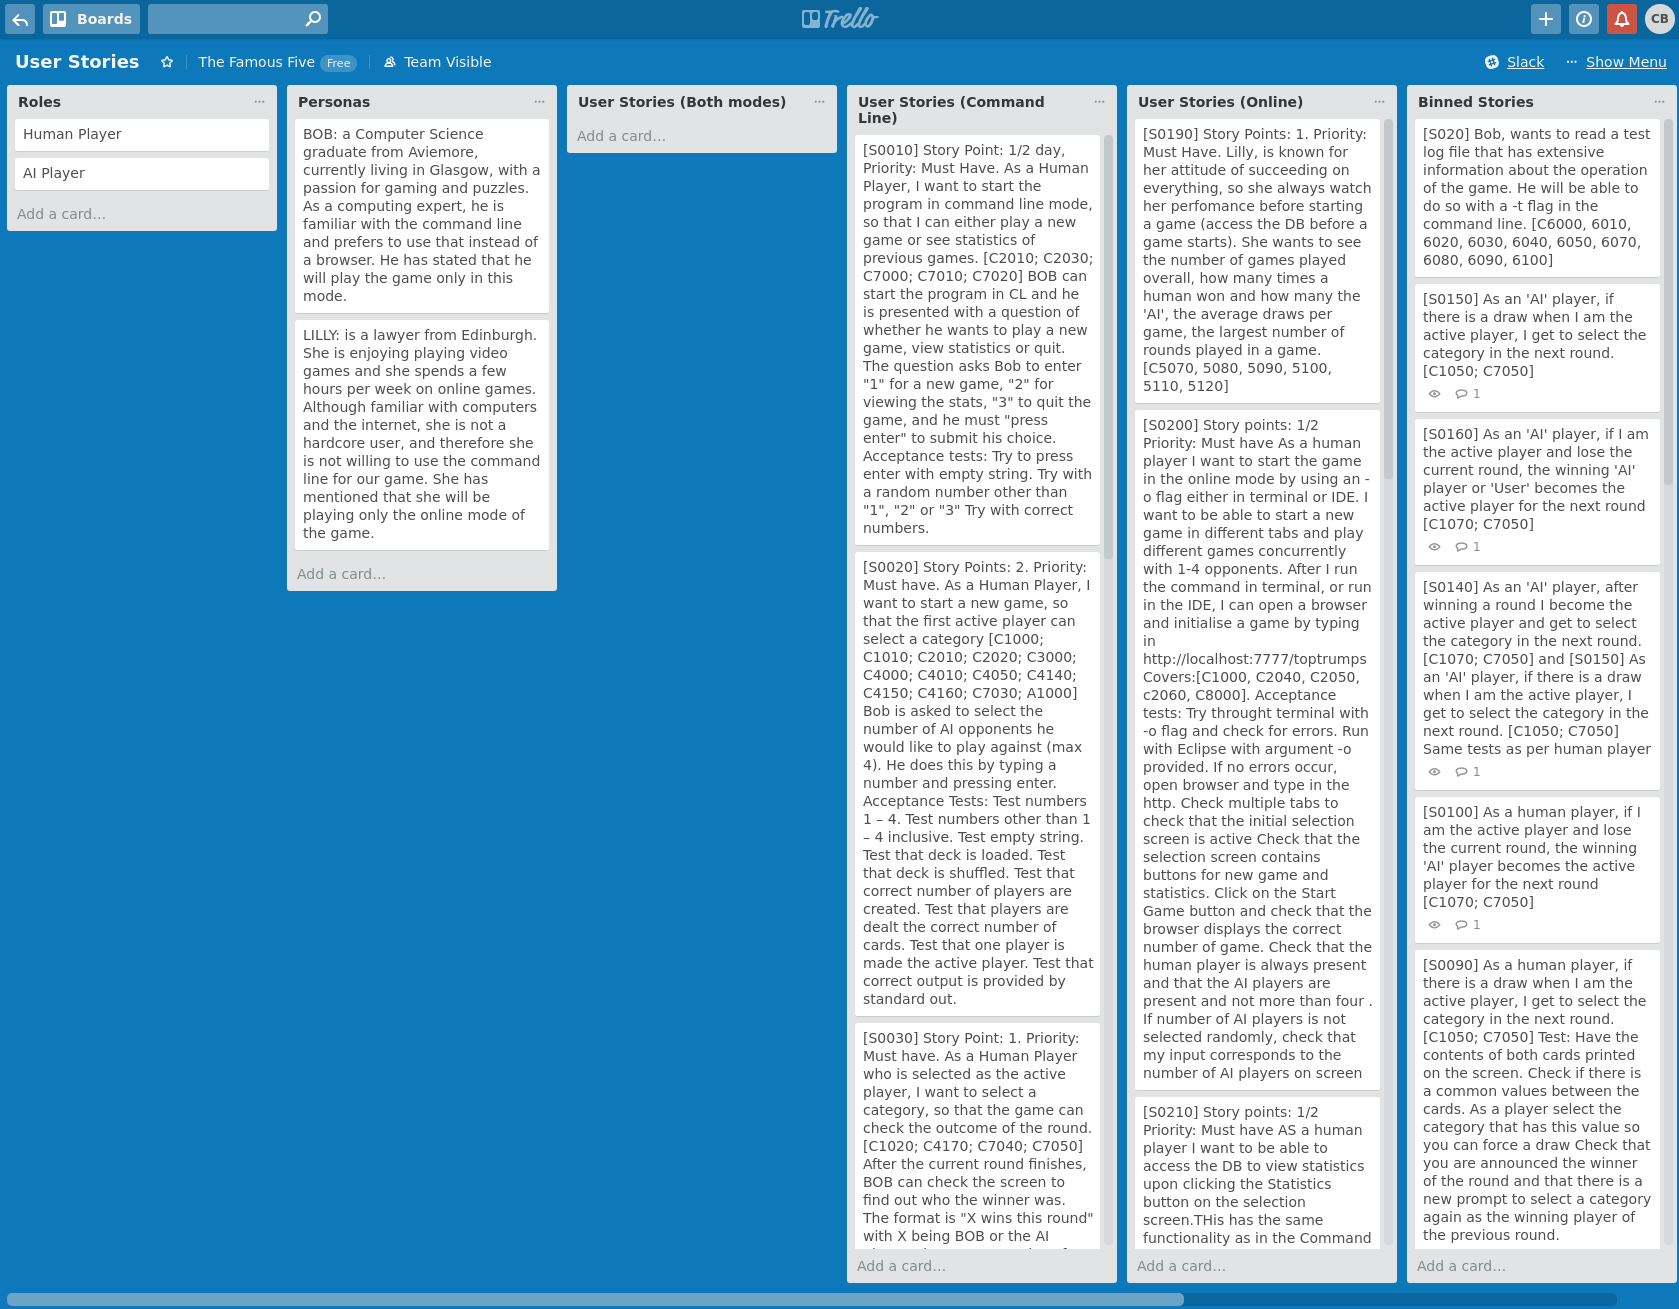
\includegraphics[scale=0.25]{user_stories_trello.png}
	\captionof{figure}{User Stories in Trello.}
	\label{fig:user_stories_trello}
\end{center}

\begin{center}
	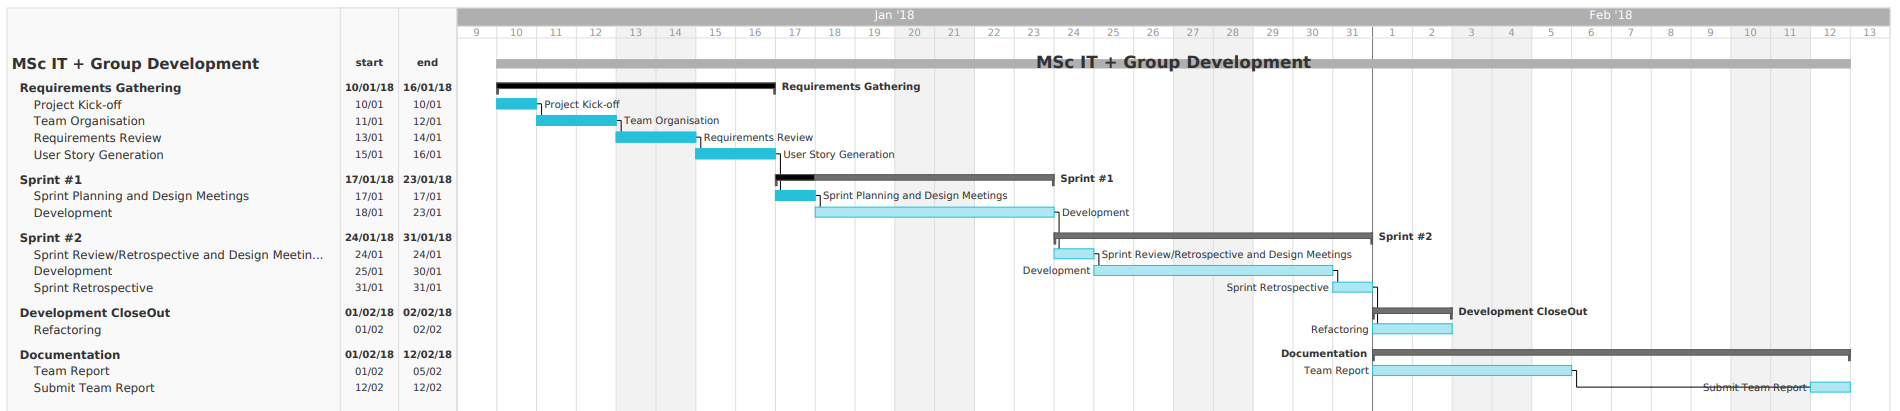
\includegraphics[scale=0.35, angle=90]{initial_project_plan}
	\captionof{figure}{Initial Project Plan}
	\label{figure:initial_project_plan}
\end{center}


\newpage
\subsection{System Design Meeting}
\label{appendix:design_meeting}

\momtoptable
{Wed 17-Jan 2018 (Week 2)}
{Slack}
{Christopher Bellingham}
{Ioannis Athanasiadis [IA]\newline
Christopher Bellingham [CB]\newline
Joseph Doogan [JD]\newline
Pavlos Evangelidis [PE]\newline
Torquil MacLeod [TM]}
{-}

\begin{momitems}
	% Item, Details, Resp., Due.
	\momitem
	{1}
	{CB provided a candidate architecture diagram (Figure \ref{figure:initial_architecture}), outlining use of an MVC architecture, with a data persistence layer. 
	CB proposed use of the Observer Pattern as a means of reducing coupling between MVC layers.}
	{INFO}
	{INFO}

	\momitem
	{2}
	{Use of the Observer Pattern was identified as a risk, since no team member has experience with this. 
	CB will outline how this would work by providing an example of a simple implementation.}
	{CB}
	{Wed 17-Jan}

	\momitem
	{3}
	{Prior to the meeting, each team member had submitted class diagrams to enable discussion on needed class structures. 
	Each submission was reviewed, and it was noted that a lot of commonality exists across proposed classes (typically Game, Player and Card classes).}
	{INFO}
	{INFO}

	\momitem
	{4}
	{CB provided detailed UML covering model and command line mode (Figures \ref{figure:initial_uml_system}, \ref{figure:initial_uml_commandline_package}, \ref{figure:initial_uml_model_package}, \ref{figure:initial_uml_persistence_package}).
	JD provided detailed UML covering online mode (Figure \ref{figure:initial_uml_online_package})
	It is understood that online mode can hook into key Game functionality via game's available public methods, and online components can be notified of game state changes via the Observer mechanism. 
	The approach as depicted was agreed to be a reasonable solution, and was selected as a basis for overall design.}
	{INFO}
	{INFO}

	\momitem
	{5}
	{CB provided detailed sequence diagram covering logical flow for command line mode (Figure \ref{figure:initial_sequence_diagram}). 
	This may be used as a reference during development.}
	{INFO}
	{INFO}

	\momitem
	{6}
	{User stories allocated to team from Appendix \ref{appendix:user_stories_command_line} to allow development to commence.}
	{INFO}
	{INFO}
\end{momitems}

\begin{center}
	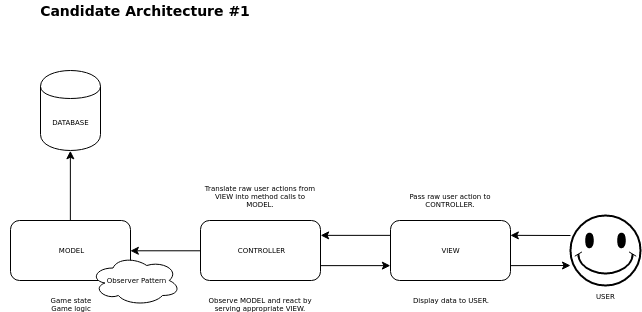
\includegraphics[width=\textwidth]{initial_architecture}
	\captionof{figure}{Proposed Architecture}
	\label{figure:initial_architecture}
\end{center}

\begin{center}
	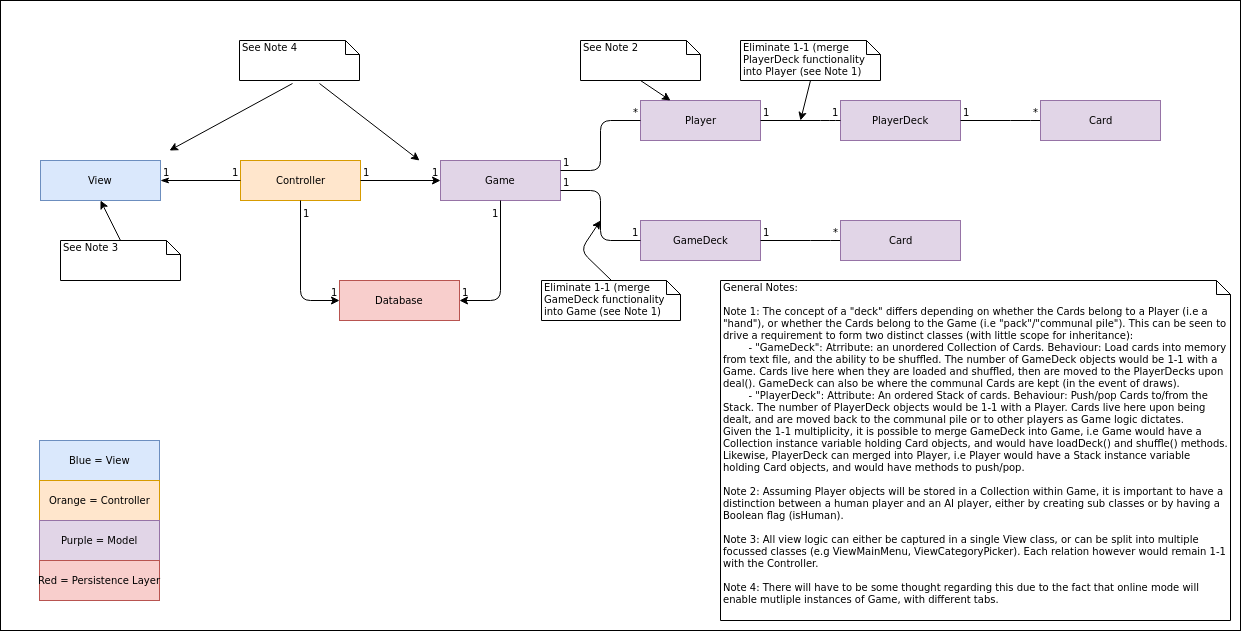
\includegraphics[width=\textwidth]{initial_uml_system}
	\captionof{figure}{Proposed System UML}
	\label{figure:initial_uml_system}
\end{center}

\begin{center}
	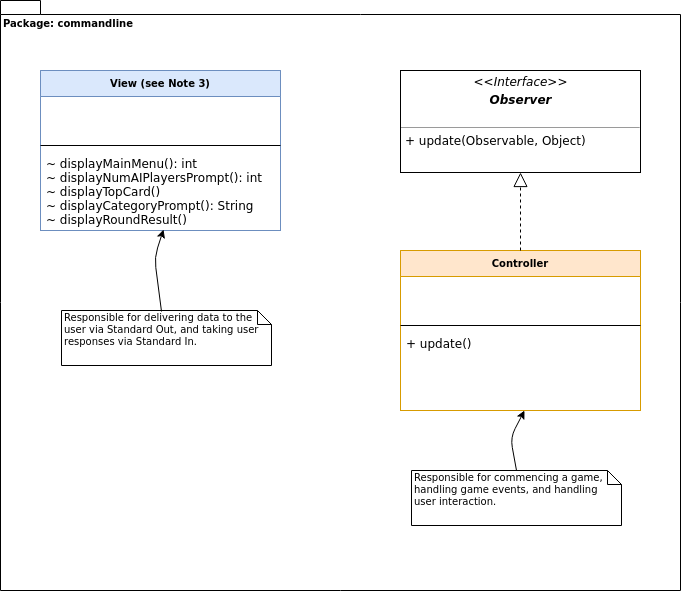
\includegraphics[width=\textwidth]{initial_uml_commandline_package}
	\captionof{figure}{Proposed Command Line Package}
	\label{figure:initial_uml_commandline_package}
\end{center}

\begin{center}
	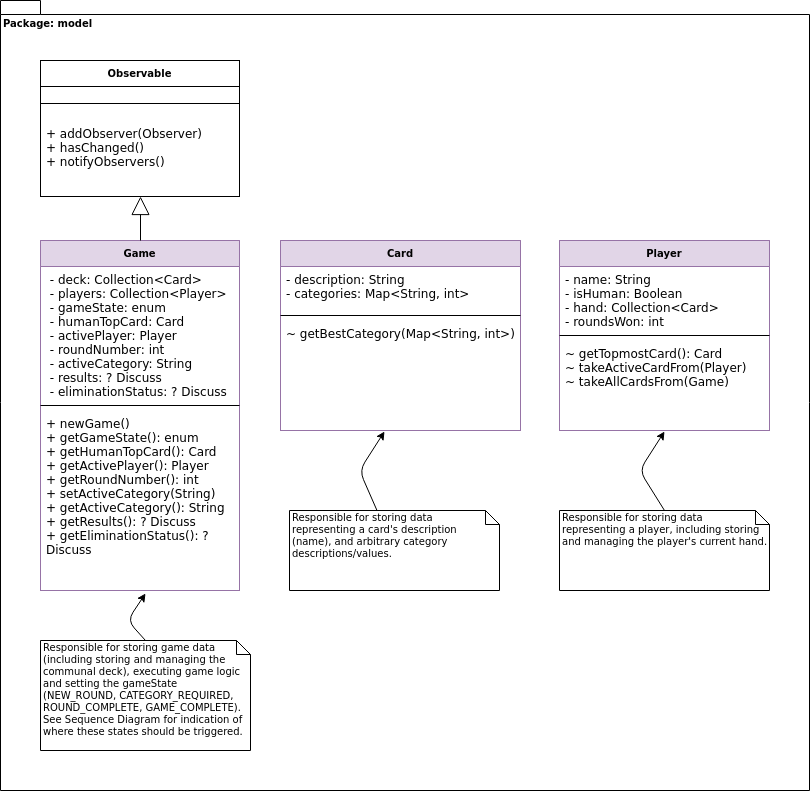
\includegraphics[width=\textwidth]{initial_uml_model_package}
	\captionof{figure}{Proposed Model Package}
	\label{figure:initial_uml_model_package}
\end{center}

\begin{center}
	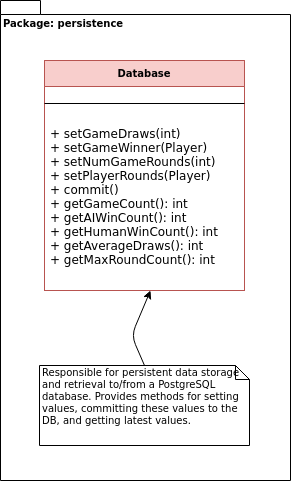
\includegraphics[scale=0.7]{initial_uml_persistence_package}
	\captionof{figure}{Proposed Persistence Package}
	\label{figure:initial_uml_persistence_package}
\end{center}

\begin{center}
	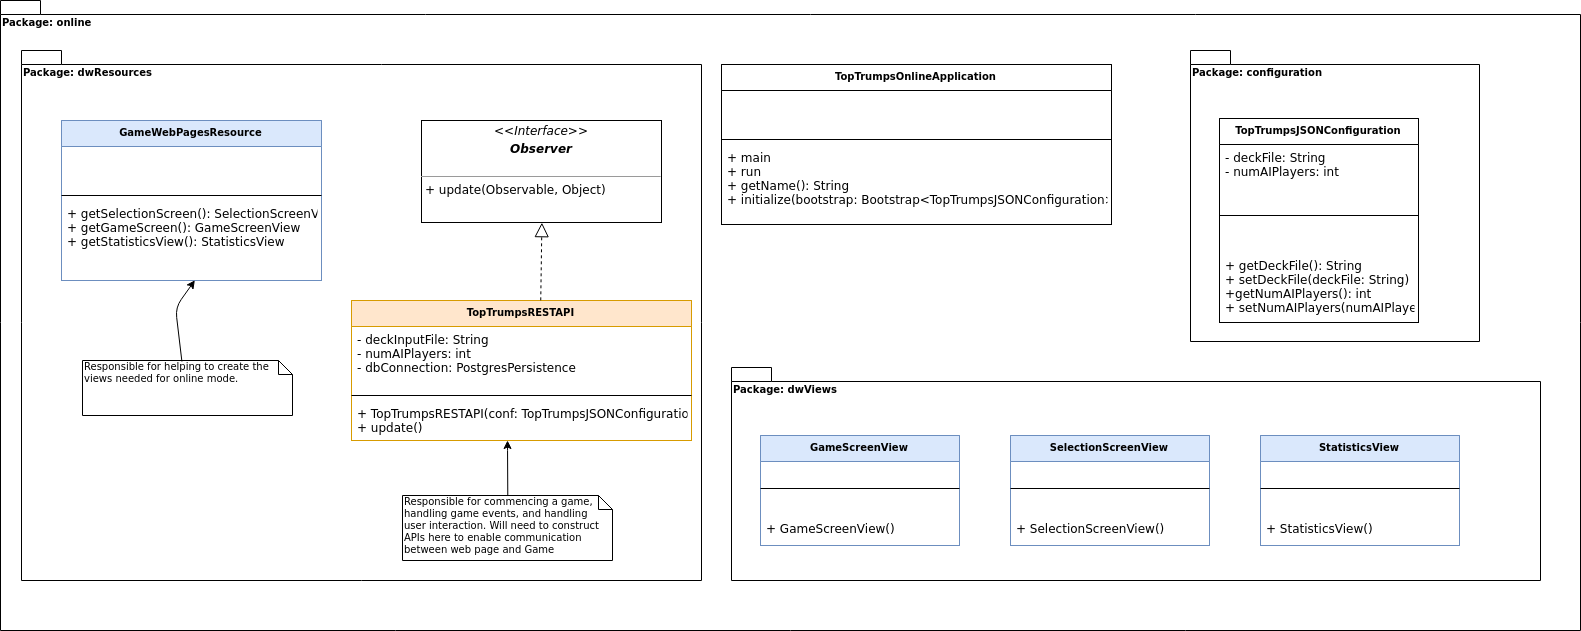
\includegraphics[width=\textwidth]{initial_uml_online_package}
	\captionof{figure}{Proposed Online Package}
	\label{figure:initial_uml_online_package}
\end{center}

\begin{center}
	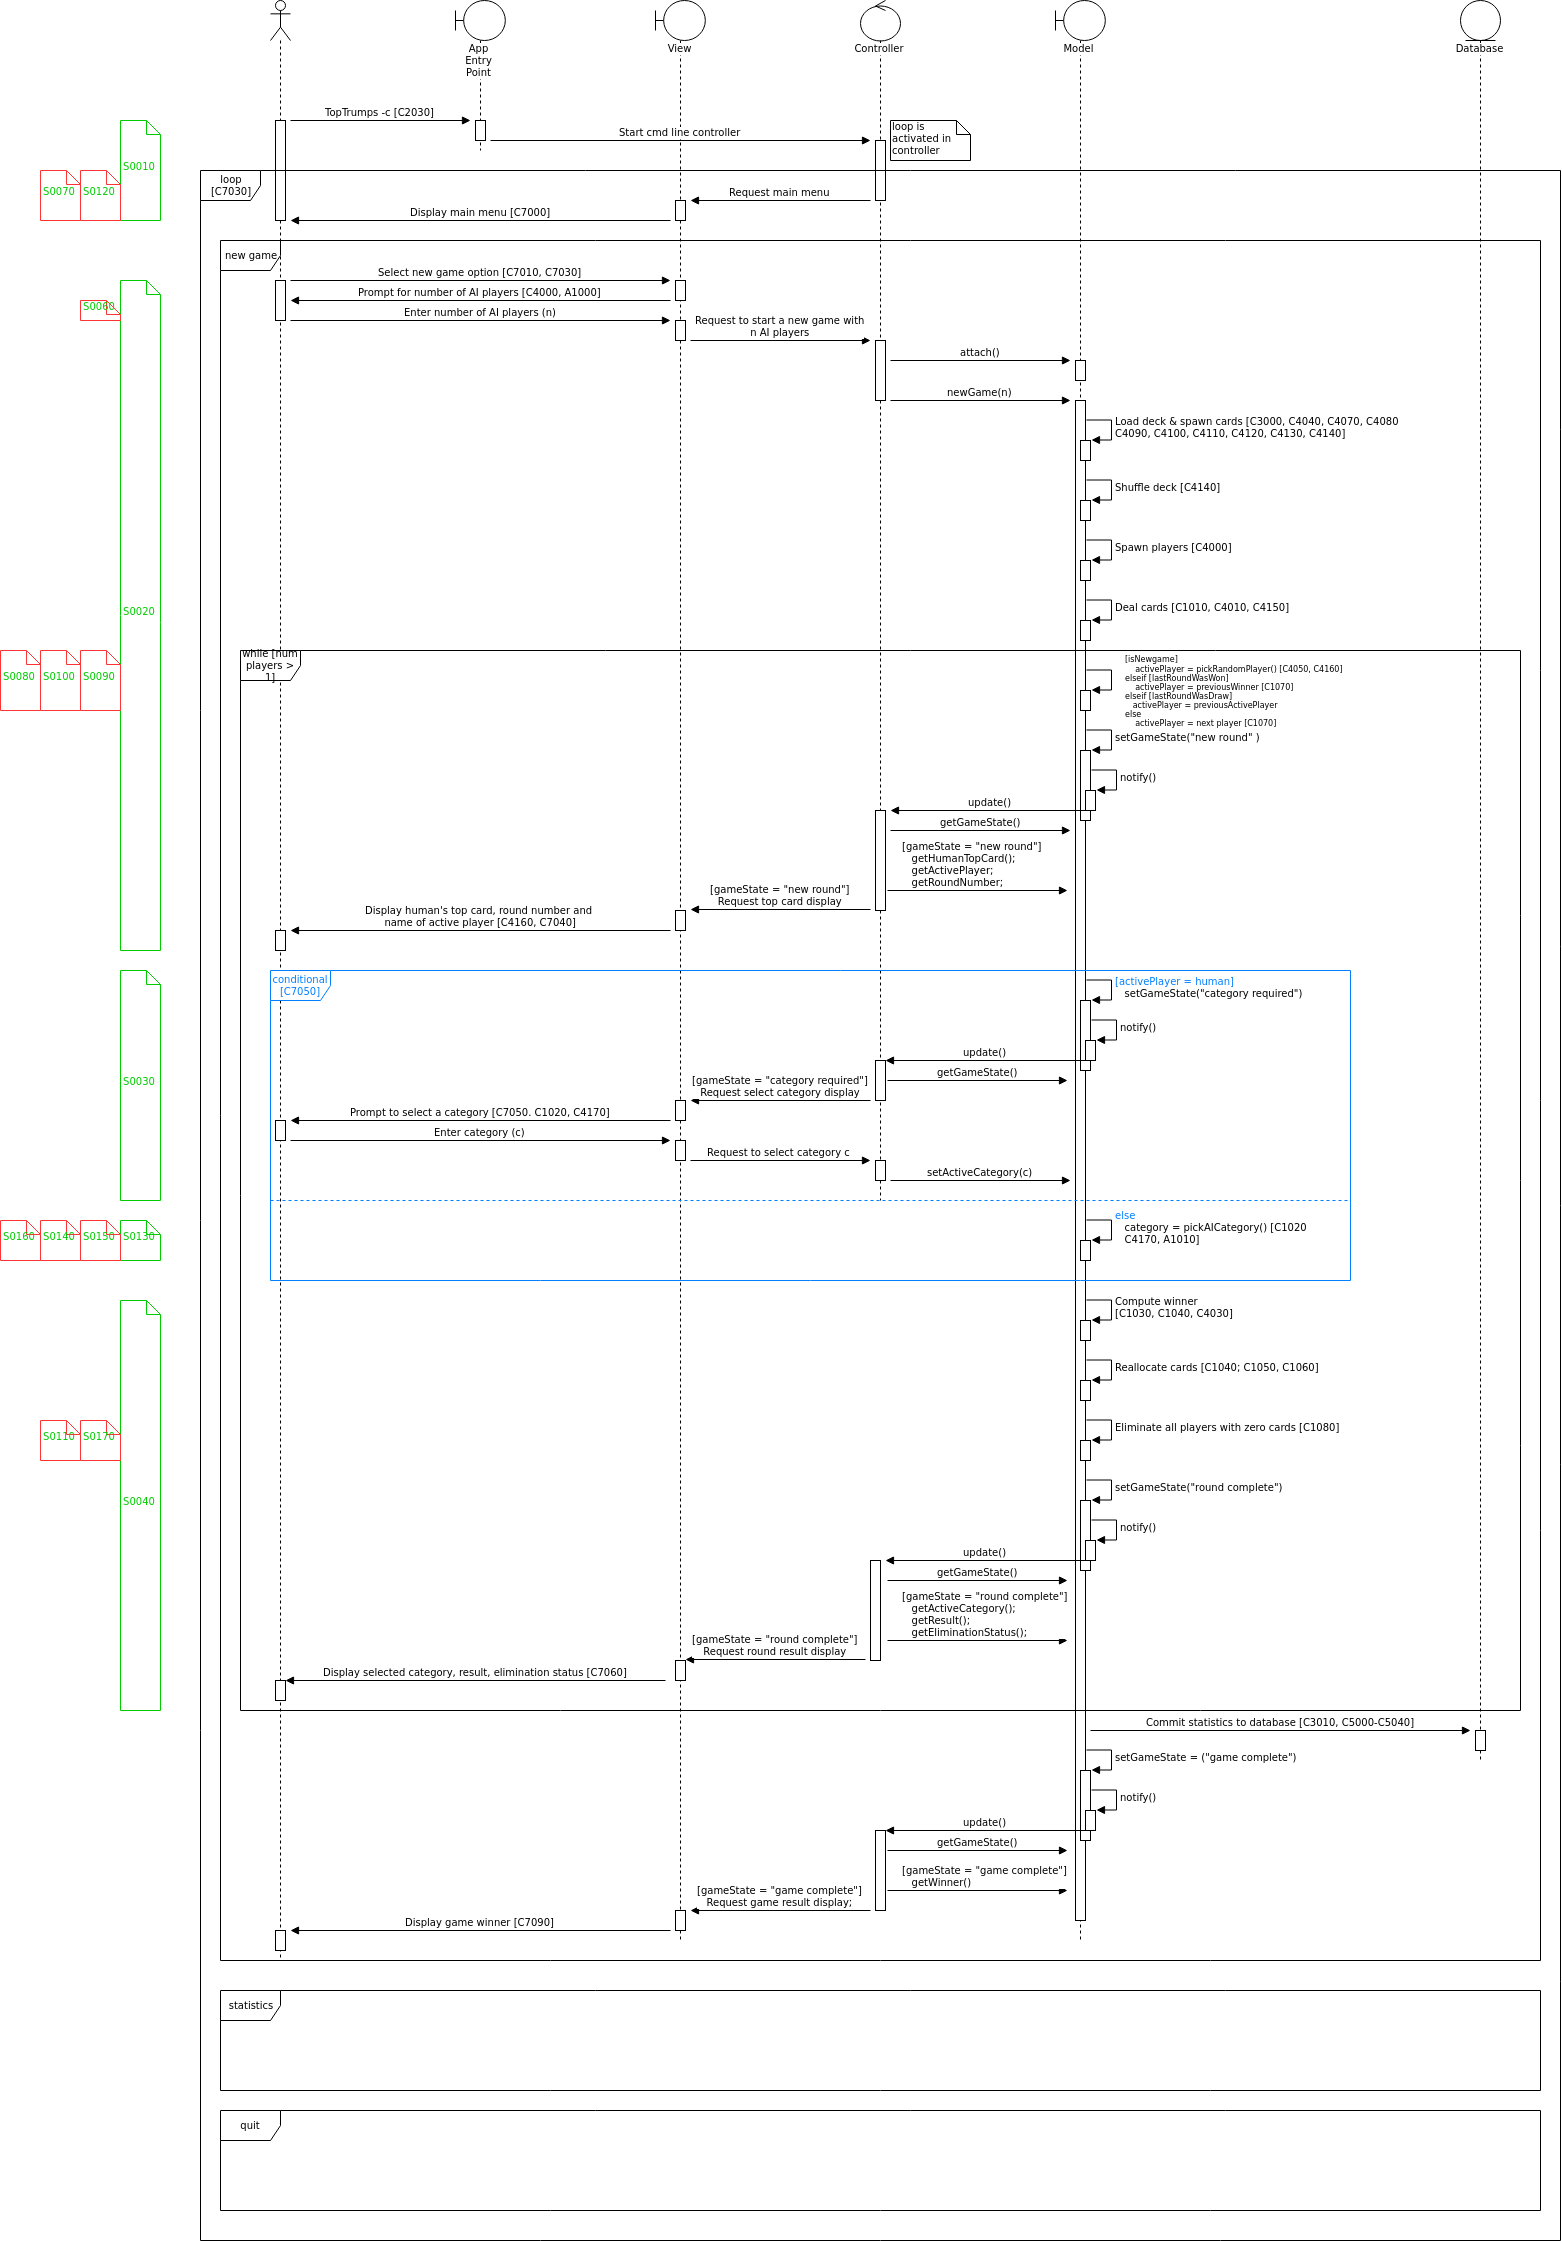
\includegraphics[scale=0.25]{initial_sequence_diagram}
	\captionof{figure}{Proposed Logical Flow}
	\label{figure:initial_sequence_diagram}
\end{center}


\newpage
\subsection{Sprint Review/Planning Meeting}
\label{appendix:sprint2_planning_meeting}

\momtoptable
{Wed 24-Jan 2018 (Week 3)}
{Slack}
{Christopher Bellingham}
{Ioannis Athanasiadis [IA]\newline
Christopher Bellingham [CB]\newline
Joseph Doogan [JD]\newline
Pavlos Evangelidis [PE]\newline
Torquil MacLeod [TM]}
{-}

\begin{momitems}
	% Item, Details, Resp., Due.
	\momitem
	{1}
	{Sprint \#1 user stories were reviewed, and it was determined that all planned stories (see Appendix \ref{appendix:user_stories_command_line}) were completed.}
	{INFO}
	{INFO}

	\momitem
	{2}
	{It was noted that initial story point estimates for S0030, S0040 and S0130 were insufficient, these took longer than expected. 
	See Appendix \ref{appendix:user_stories_command_line} for actual durations. 
	This was due to unexpected underlying complexities, and the need to build-out the initial underlying program structure in order to implement these features.}
	{INFO}
	{INFO}

	\momitem
	{3}
	{Team feels that the workflow, particularly use of Slack to communicate, has been effective. 
	No changes to process are deemed necessary.}
	{INFO}
	{INFO}

	\momitem
	{4}
	{Discussion moved onto Sprint \#2, where the stories in Appendix \ref{appendix:user_stories_online} were reviewed.
	Ref item [2], to learn lessons from Sprint \#1 overrun, the story points allocated to Sprint \#2 stories were increased, specifically stories S0200, S0220 and S0230).
	This is in recognition of technology risk, as no team member has experience with Dropwizard, and only limited experience with HTML/CSS.
	The assumption remains that the underlying Model logic components developed in Sprint \#1 can be re-used however.}
	{INFO}
	{INFO}

	\momitem
	{5}
	{Based on sum of all proposed Sprint \#2 stories, velocity for this sprint increases from originally planned 7 to 10.
	Team feel able to meet the increased workload.}
	{INFO}
	{INFO}

	\momitem
	{6}
	{Project schedule was presented, updated to show latest progress. 6 days still remain for float/contingency prior to report submission (Figure \ref{figure:sprint2_project_plan}).}
	{INFO}
	{INFO}

	\momitem
	{7}
	{User stories allocated to team from Appendix \ref{appendix:user_stories_online} to allow development to commence.}
	{INFO}
	{INFO}
\end{momitems}

\begin{center}
	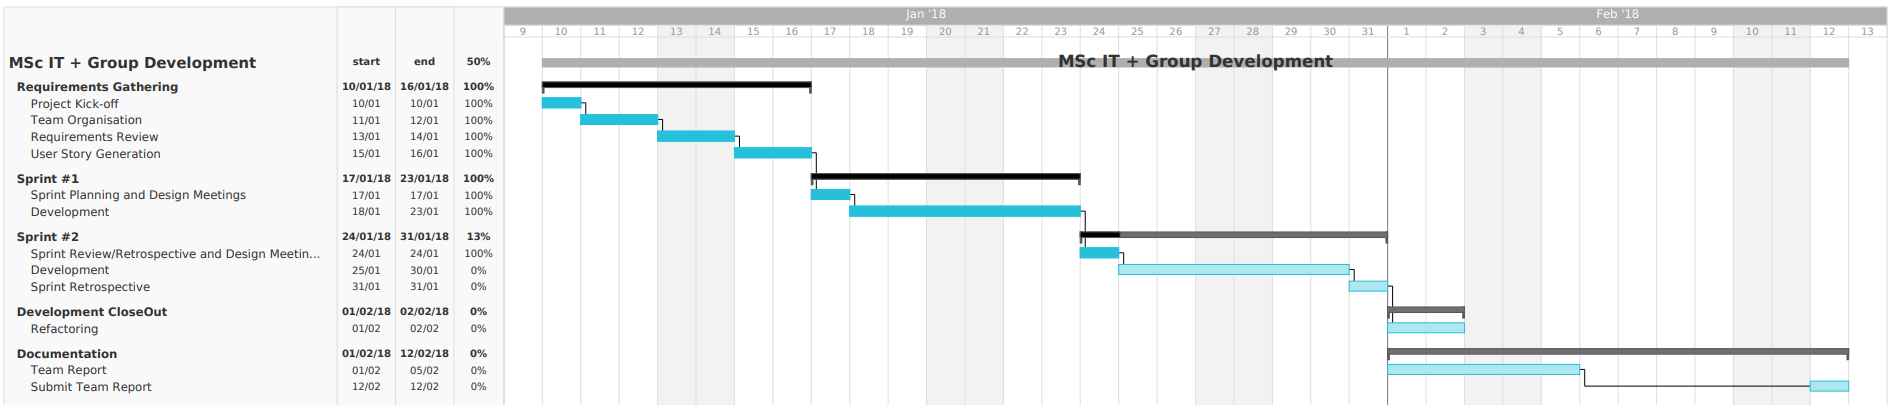
\includegraphics[scale=0.35, angle=90]{sprint2_project_plan}
	\captionof{figure}{Project Plan prior to Sprint \#2.}
	\label{figure:sprint2_project_plan}
\end{center}


\newpage
\subsection{Sprint Review/Planning Meeting}
\label{appendix:sprint3_planning_meeting}

\momtoptable
{Wed 31-Jan 2018 (Week 4)}
{Slack}
{Christopher Bellingham}
{Ioannis Athanasiadis [IA]\newline
Christopher Bellingham [CB]\newline
Joseph Doogan [JD]\newline
Pavlos Evangelidis [PE]\newline
Torquil MacLeod [TM]}
{-}

\begin{momitems}
	% Item, Details, Resp., Due.
	\momitem
	{1}
	{Sprint \#2 user stories were reviewed, and it was determined that not all planned stories (see Appendix \ref{appendix:user_stories_online}) were completed. Stories S0220, S0230, S0240 and S0250 remain incomplete.}
	{INFO}
	{INFO}

	\momitem
	{2}
	{Lack of team experience with the online technologies is responsible for the overrun. 
	The asynchronous and stateless nature of the API calls was not considered during design stage. Some additional work is needed to refactor the underlying model to suit the online technologies.}
	{INFO}
	{INFO}

	\momitem
	{3}
	{A third sprint must be scheduled to cover refactoring and to allow completion of stories S0220, S0230, S0240 and S0250.}
	{INFO}
	{INFO}

	\momitem
	{4}
	{A revised project plan is proposed, making use of the available schedule float (Figure \ref{figure:sprint3_project_plan}).}
	{INFO}
	{INFO}

	\momitem
	{5}
	{Durations for user stories S0220, S0230, S0240 and S0250 adjusted to capture required refactoring.
	See Appendix \ref{appendix:user_stories_online_additional}.}
	{INFO}
	{INFO}

	\momitem
	{6}
	{Based on sum of all proposed Sprint \#3 stories, velocity for this sprint is 11.
	Team feel able to meet the increased workload.}
	{INFO}
	{INFO}

	\momitem
	{7}
	{Duration for team report is extended to account for reduced available resources.
	Report can be written in parallel with Sprint \#3, and extended over the final weekend (Figure \ref{figure:sprint3_project_plan}).}
	{INFO}
	{INFO}

	\momitem
	{8}
	{User stories allocated to team from Appendix \ref{appendix:user_stories_online_additional} to allow development to commence.}
	{INFO}
	{INFO}
\end{momitems}

\begin{center}
	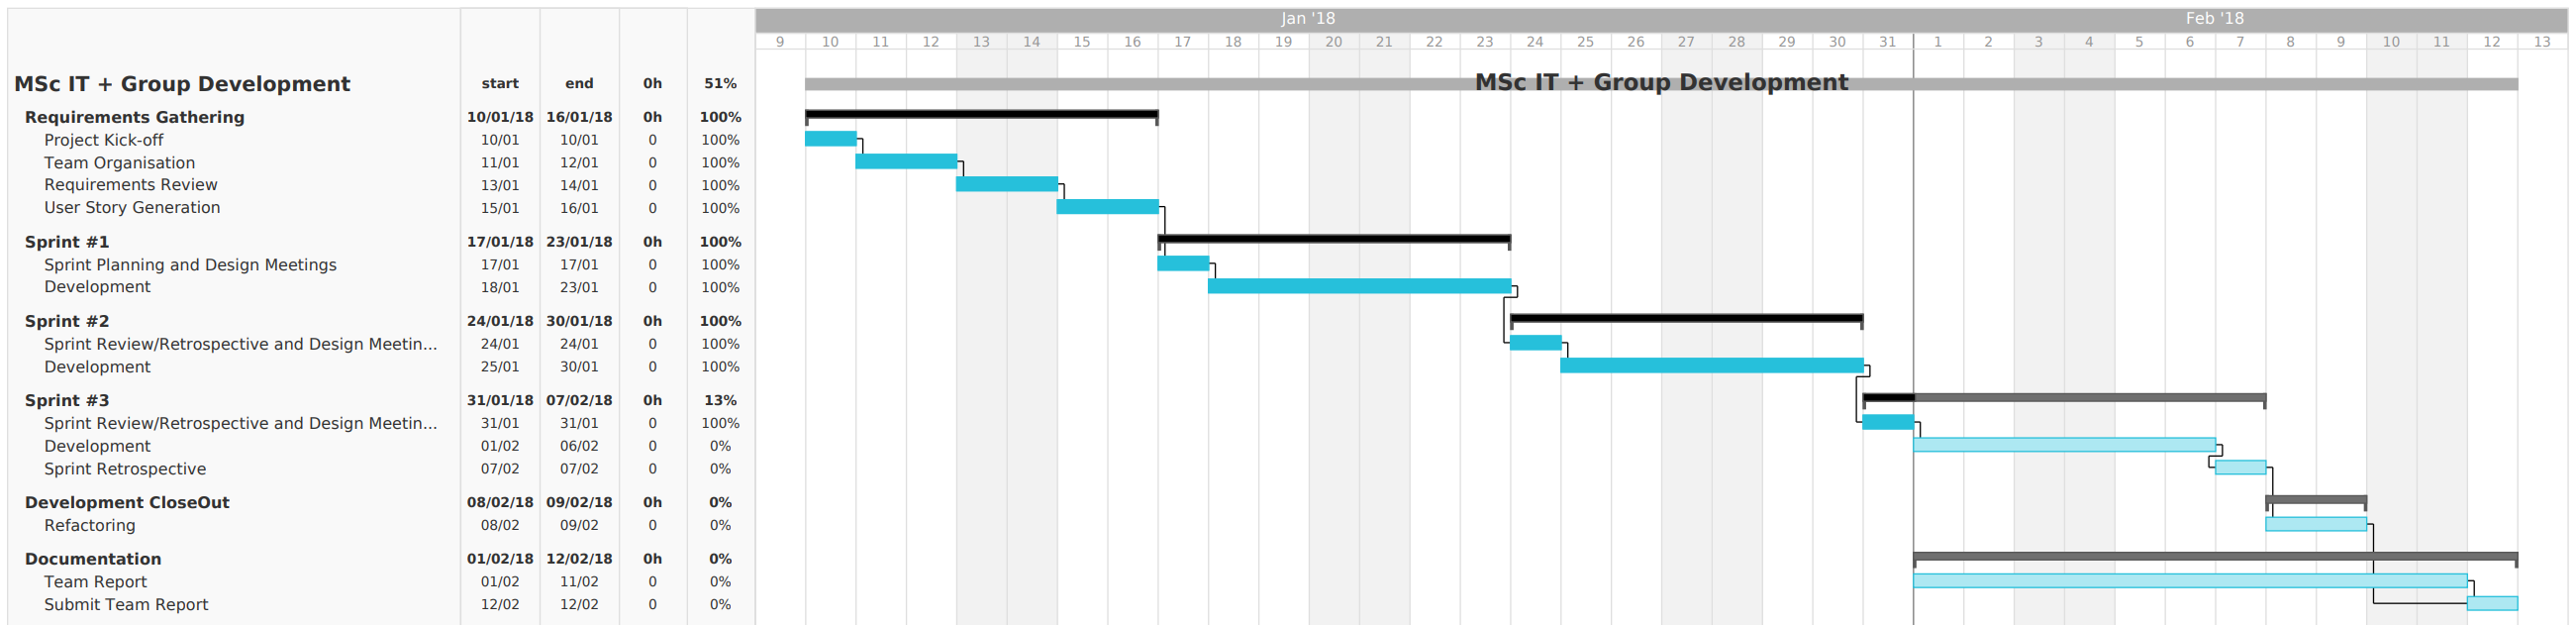
\includegraphics[scale=0.25, angle=90]{sprint3_project_plan}
	\captionof{figure}{Project Plan prior to Sprint \#3.}
	\label{figure:sprint3_project_plan}
\end{center}


\newpage
\subsection{Sprint Retrospective}
\label{appendix:final_sprint_meeting}

\momtoptable
{Wed 07-Feb 2018 (Week 5)}
{Slack}
{Christopher Bellingham}
{Ioannis Athanasiadis [IA]\newline
Christopher Bellingham [CB]\newline
Joseph Doogan [JD]\newline
Pavlos Evangelidis [PE]\newline
Torquil MacLeod [TM]}
{-}

\begin{momitems}
	% Item, Details, Resp., Due.
	\momitem
	{1}
	{Sprint \#3 user stories were reviewed, and it was determined that all planned stories (see Appendix \ref{appendix:user_stories_online_additional}) were completed.}
	{INFO}
	{INFO}

	\momitem
	{2}
	{All stories were completed in-line with their expected durations. For latest project plan see \ref{figure:final_project_plan}.}
	{INFO}
	{INFO}
	
	\momitem
	{3}
	{Opportunity will be taken by all team members to review all code and tidy-up prior to submission.}
	{INFO}
	{INFO}

	\momitem
	{4}
	{Final testing will be performed in the Boyd Orr Lab, Thurs 08-Feb, including testing the database functionality on the Yacata server.
	All team members will present in the Lab to support any issues.}
	{ALL}
	{INFO}
\end{momitems}

\begin{center}
	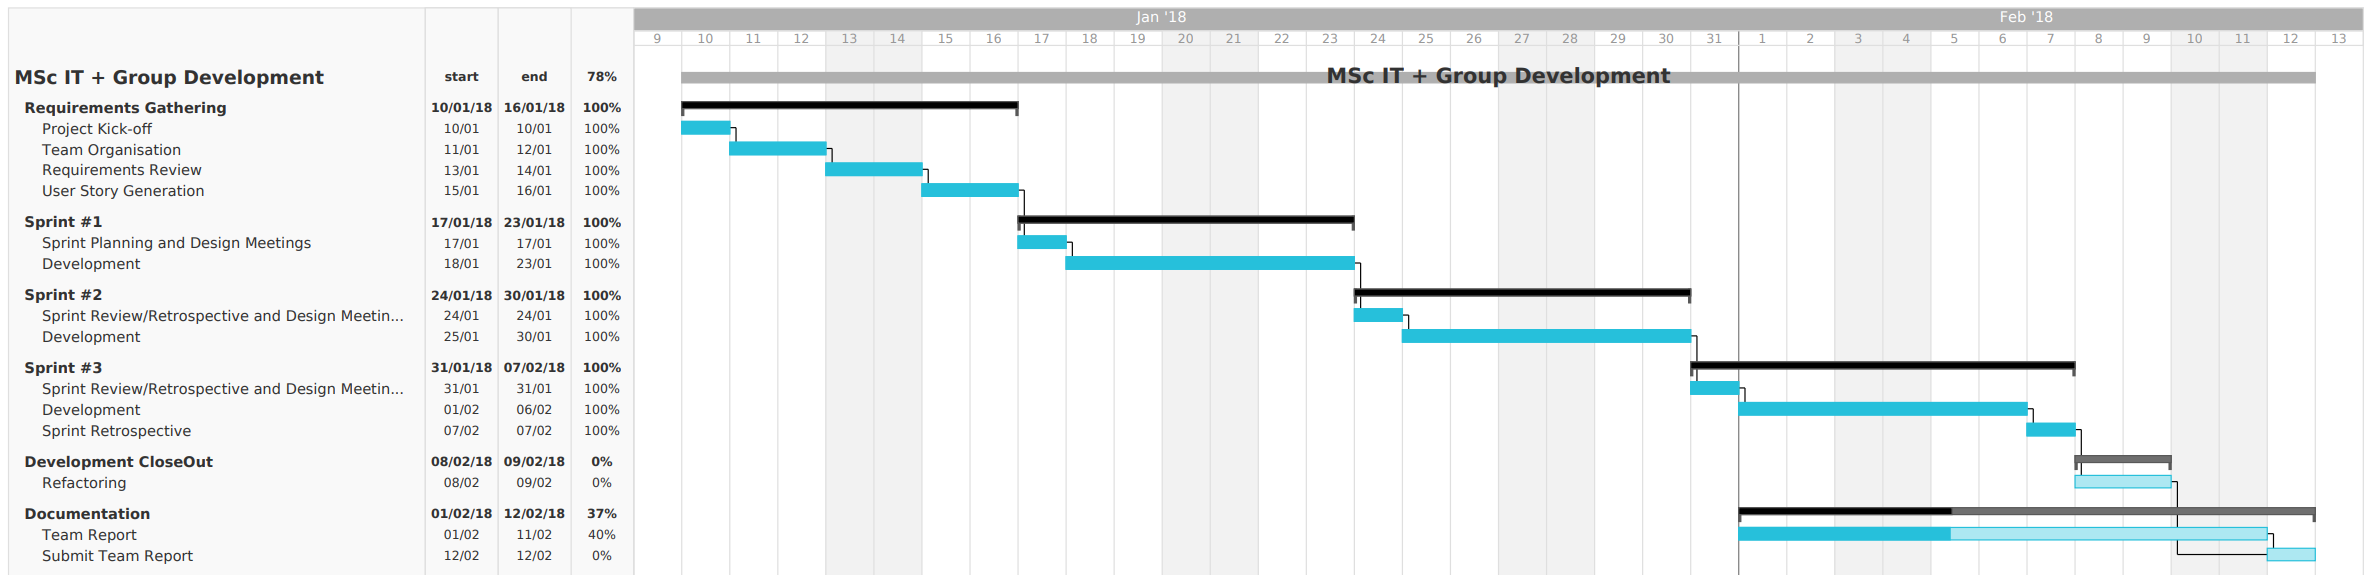
\includegraphics[scale=0.25, angle=90]{last_project_plan}
	\captionof{figure}{Project Plan at Sprint \#3 completion.}
	\label{figure:final_project_plan}
\end{center}